\chapter{Power Measurement}

\section{Validating RAPL Accuracy}
Since the Haswell microarchitecture Intel integrated current measurement 

\todoms{Cite the rapl papers (haswell, alderlake). One doctoral thesis about the ice lake processor.}
\todoms{Robert: Auf capella messen. nur square fit, abwechselnd die sockets populieren}

\begin{figure}[]
    \centering
    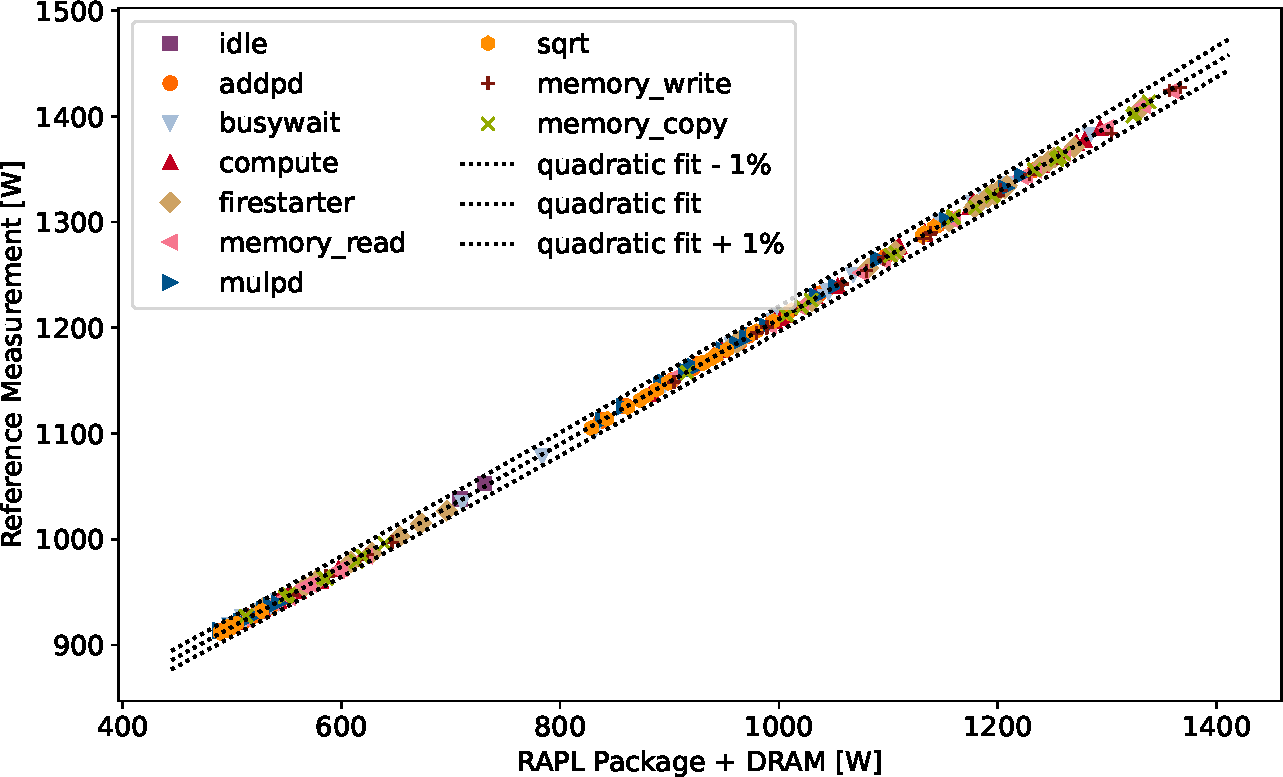
\includegraphics[width=\columnwidth]{fig/rapl-validation.pdf}
    \caption{\label{fig:validate-rapl}The roco2 microbenchmark is executed on a varying number of cores with different frequencies.
    We can validate the accuracy of RAPL with the quadratic fit between the external measurement and the RAPL measurement.
    We do not replicate the findings of Alderlake.}
\end{figure}

\section{RAPL Filters}
